\chapter{Вычислительно эффективный алгебраический метод восстановления FHT-SIRT} \label{chapt1}

\section{Введение}

В данной главе предложен и обсуждается асимптотически быстрый алгоритм SART \cite{sart}, основанный на реализации быстрого преобразования Хафа (БПХ) \cite{hough}.
Алгоритм решает задачу восстановления для случая зондирования монохроматическим параллельным излучением.
Требуемое доказательство асимптотической оценки сложности алгоритма представлено.
Численная реализация алгоритма проиллюстрирована результатами реконструкции модельного изображения размером 256 $\times$ 256 по полному набору 1021 углов БПХ и по разреженным синограммам, имеющим до 11 раз меньшее число проекционных углов.

\section{Алгебраический подход}
Одна из отличительных особенностей алгебраического метода --- переход к дискретному представлению сущностей в задаче на в самом начале решения задачи. 
Дискретное представление изображения $\textbf f$ будет удобно обозначать с двумя индексациями: линейной ($f_j$) и матричной ($f_{kl}$). 
Матричная форма удобна для восприятия характеристики $\textbf f$ как двумерного изображения с пространственными значением координат.
Линейная форма же удобна при работе с изображением как с элементом линейного пространства.
Хотя существует множество способов отображения двумерных пространственных координат в одномерный индекс, конкретный способ линейной индексации не имеет значения в дальнейших выкладках.
Из соображений простоты и определенности, можно считать, что изображения-столбцы индексируются в порядке инексации матричных осей, т.е. по строкам слева-направо ($j = k * n + l$, при размере изображения $n$ и индексации, начинаемой с 1).

Радоновское проецирование дискретного изображения может быть представлено в виде действия линейного оператора
\begin{equation}\label{eq:linear_system}
\textbf p = W \textbf f,
\end{equation}
где $\textbf p$ --- прологарифмированная и отнормированная синограмма, $\textbf f$ --- искомое изображение, а элемент $w_{ij}$ матрицы $W$ соответствует вкладу $i$-го пикселя в $j$-ый луч.
Коэффициенты $0 \leq w_{ij} \leq 1$ могут задаваться по-разному, например так:
\begin{equation}
\label{eq:coeff}
w_{ij} = \frac{\text{Площадь пикселя $i$, перекрываемая лучом $j$}}{\text{площадь пикселя $i$}}
\end{equation}
Вид матрицы $W$ задает оператор проектирования, используемый при восстановлении.
От оператора проектирования зависит поведение алгоритма восстановления.

В дальнейшем изложении будет использовано разложение матрицы $W$ и проекционных данных $\textbf p$ на составляющие, соответствующие определенному углу:
\begin{equation} \notag
\begin{array}{l l}
w_{ij} = \sum_{h = 1}^{M_\varphi} {w_{ij}^{\varphi(h)}}, & \quad
p_i = \sum_{h = 1}^{M_\varphi} {p_i^{\varphi(h)}}.
\end{array}
\end{equation}
Здесь $M_\varphi$ ---  полное число проекционных углов в синограмме, а  $w_{ij}^{\varphi(h)}$ и $p_i^{\varphi(h)}$ учитывают только лучи, направленные по углу с номером $h$ (т. е. элементы, не относящиеся к углу $h$, равны нулю).

\section{Метод восстановления ART}
\label{ss:SART}
В алгебраическом методе (ART) изображение восстанавливается с помощью итерационного процесса:
\begin{enumerate}
\item{задается начальное приближение --- 2D кусочно-постоянная функция $\textbf f^{(0)}$ , которая описывает распределение коэффициента ослабления;}
\item{рассчитывается \textbf{одна} лучевая сумма вдоль одного из направлений $(W\textbf f)_i$, где $i$ --- индекс синограммы, соответствующий выбранному направлению;}
\item{отличие значения величины точки на проекции от рассчитанной величины лучевой суммы распределяется с учетом весовых коэффициентов между всеми пикселями, определившими направление, формируя добавку $(\textbf p - W \textbf f)_i$;}
\item{добавка, взвешенная релаксационным параметром \cite{art_regparam}, суммируется с текущим значением 2D кусочно-постоянной функции:
  \begin{equation} \label{eq:art_it}
\begin{array}{l l}
    \mathrm f^{(\text{нов})}_j = \mathrm f_j + \gamma w_{ij}\frac{(\textbf p - W \textbf f)_i}{\sqrt{\sum_k {w_{ik}^2}}}, & \quad j \in \overline{1, N},
\end{array}
  \end{equation}

где $N = M_s \cdot M_s$ --- полное количество пикселей в восстанавливаемом изображении, а $M_s$ --- полное количество сдвигов луча (полное количество делений линейного детектора).}
\end{enumerate}
Шаги 2 --- 4 повторяются для следующего выбранного направления. 
Итерация считается законченной, когда операция выполнена для всех направлений.
Новая итерация повторяет шаги 2 --- 4. Итерационная процедура заканчивается согласно выбранному критерию останова.
Схема перебора точек на проекциях может быть различной \cite{art_pointschoice}.  

Существуют разные вариации метода ART.
Для дальнейшего повествования потребуется метод SART, отличающийся от обычного ART тем, что на одной итерации невязка вычисляется сразу по всем точкам синограммы, а после этого в изображение вносится одна большая поправка.
Таким образом, итерационный процесс будет иметь вид
\begin{equation} \label{eq:sart_it_1}
  \textbf f^{(\text{нов})} = \textbf f + \gamma{W}^\mathrm{T}\frac{\textbf{p} - W \textbf f}{\sqrt{\sum_{i,j} {w_{ij}^2}}},
\end{equation}  
где за ${W}^\mathrm{T}$ обозначено транспонирование матрицы $W$.

\section{Геометрическое описание итерации}
Полезно представлять геометрически, что происходит с изображением при одном шаге алгоритмов ART и SART.
Если начальным приближением было абсолютно черное изображение ($\textbf f^{(0)} = 0$), то после одной итерации ART при суммировании (\ref{eq:art_it}) изменяются лишь пиксели, соответствовавшие некоторому лучу.
Результирующее изображение будет черным и будет содержать только одну полосу, причем яркость пикселей в этой полосе будет пропорциональна весам. 

При учете всей проекции по некоторому углу $\varphi$ результирующее изображение может быть получено следующим способом.
Рассмотрим некоторую строчку $h$ синограммы, соответствующую углу $h \leftrightarrow \varphi$. Введем обозначения: 
\begin{equation}\label{eq:misalligment}
\begin{array}{l l}
q^\varphi_l = (\textbf p - W \textbf f)_{hl},& \quad l \in \overline{1, M_s}, \\
r^\varphi_{kl} = q^\varphi_l, & \quad k,l \in \overline{1, M_s}.
\end{array}
\end{equation}
В этой формуле $q^\varphi_l$ --- строка длины $M_s$, соответствующая невязке синограммы по углу $\varphi$ на текущей итерации; $r^\varphi_{kl}$ --- изображение размера $M_s \cdot M_s$, постоянное вдоль столбцов, причем каждая строка этого изображения равна $q^\varphi_l$.
Все лучи, соответствующие одному углу, считаем пронумерованными в порядке их отступа вправо.
Чтобы получить финальную поправку на текущей итерации, нужно повернуть изображение $\textbf r^\varphi$ на угол $\varphi$ и прибавить к исходному, умножив предварительно на релаксационный параметр $\gamma$.
Обозначим описанную процедуру так:
\begin{equation}
\label{eq:geometric_sart_it}
\textbf f = \textbf f^{(0)} +\gamma\cdot\text{\textrm{повернуть}}(\textbf r^\varphi, \varphi).
\end{equation}
Сравнивая вид (\ref{eq:sart_it_1}) и (\ref{eq:geometric_sart_it}), можно заключить, что
\begin{equation}
\label{eq:alg_geom_conn}
{W^\varphi}^{\mathrm T}(\textbf p - W \textbf f) = \text{\textrm{повернуть}}( \textbf r^\varphi, \varphi).
\end{equation}

\section{Применение преобразования Хафа}
Принципиальное различие между интегральным и алгебраическим подходами к восстановлению в томографии состоит в следующем.
Результаты работы методов одинаковы --- дискретное изображение, соответствующее просвечиваемому объекту.
Однако алгоритмы, основанные на интегральном подходе, считают восстанавливаемую функцию непрерывной вплоть до этапа вычислений, а алгебраические методы работают с дискретным изображением (кусочно-постоянной функцией) уже на этапе постановки задачи.

Аналогично, было предложено пойти дальше и заменить модель, которая наилучшим образом приближает лучи с физической точки зрения, на модель дискретных симметричных лучей-ступенек, позволяющую производить быстрые вычисления.
Такое приближение известно как \textbf{быстрое преобразование Хафа}.

Быстрое преобразование Хафа (БПХ) изображения $\textbf f$ размера $n \cdot  m$ --- это изображение $\textbf p$ размера не более чем $2(n+m) \cdot (n+m)$, в каждой ячейке которого хранится сумма пикселей $\textbf f$ вдоль соответствующих лучей; по строкам располагаются суммы вдоль лучей с одинаковым углом наклона, а по столбцам --- с одинаковым отступом.
Преобразование Хафа является дискретным аналогом преобразования Радона (см. рис. \ref{fig:hough_radon}).

\begin{figure}[h!]
  \centering
    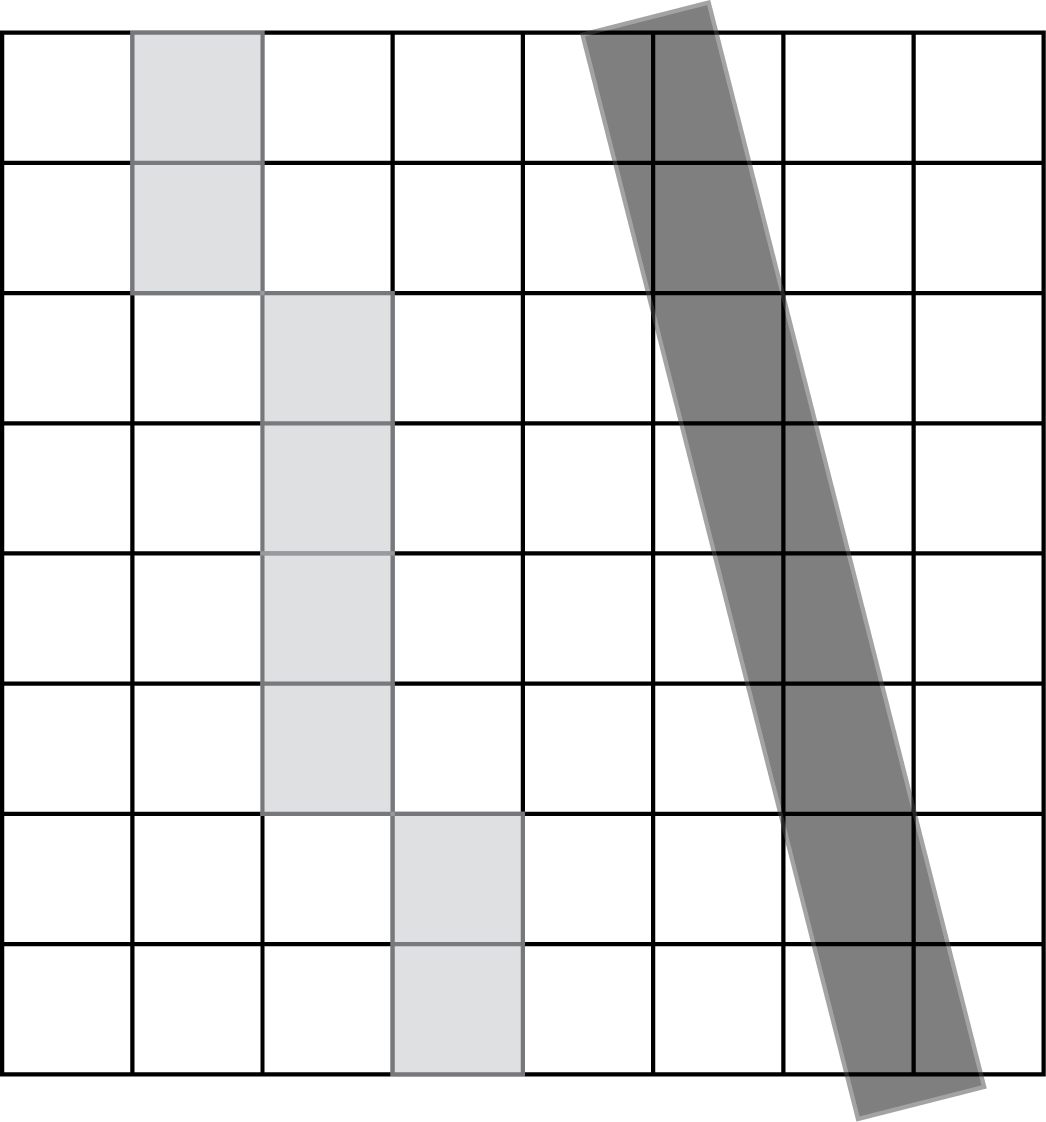
\includegraphics[width=0.55\textwidth]{part1_img/ART-Discr-ru}
 \caption{Различия в представлении лучей.}
Слева --- луч в БПХ, справа --- некоторе приближение бесконечно тонкого луча.
\label{fig:hough_radon}
\end{figure}

Полное преобразование Хафа изображения можно считать быстро за $O(n^2\log n)$, где $n$ --- линейный размер изображения.
Подробнее о быстром преобразовании Хафа можно прочитать в \cite{hough}.
Далее речь будет идти только о БПХ.

\section{Изменение в итерации}
Для построения алгоритма восстановления томографии, использующего преобразование Хафа в качестве оператора получения синограммы изображения, возьмем за основу алгоритм, описанный в разделе \ref{ss:SART}.
Полная накопленная поправка имеет вид
\begin{equation}
\label{eq:sum}
\Delta \textbf f = \sum_\varphi {{W^\varphi}^{\mathrm T}(\textbf p - W\textbf f) } = W^{\mathrm T}(\textbf p - W \textbf f).
\end{equation}
При использовании преобразования Хафа матрица $W$ становится заполненной только нулями и единицами в соответствии с паттернами углов, приближающих лучи.
Здесь и далее будем считать, что синограмма $\textbf p$ представлена в координатах пространства БПХ.
\subsection{Обоснование сходимости}
Рассмотрим функционал невязки
\begin{equation}
Q(\textbf f ) = ( W\textbf f - \textbf p)^2,
\end{equation}
где $W$ --- матрица весов.
Очевидно, что $Q( \hat{\textbf f}) = 0$, если $\hat{\textbf  f}$ --- восстанавливаемое изображение.
Найдем минимум функционала $Q$ методом градиентного спуска:
\begin{equation}
\nabla Q = 2 W^\mathrm{T}(W\textbf f - \textbf P).
\end{equation}
Шаг градиентного спуска выглядит так:
\begin{equation}
\label{eq:gradient_decay}
\textbf f^{(n)} = \textbf f^{(n-1)} - \gamma  W^\mathrm{T}(W\textbf f - \textbf p).
\end{equation}
Последнее уравнение соответствует итерационной процедуре (\ref{eq:sart_it_1}) с точностью до нормировки весовых коэффициентов.
%но это не имеет значения в случае использования преобразования Хафа, так как там нормы всех весовых коэффициентов одинаковы и могут быть включены в релаксационный параметр $\gamma$.

\subsection{Улучшение асимптотики}
Далее покажем, как улучшить асимптотику одной итерации с $O(n^3)$ до $O(n^2 \log n)$, где $n$ --- линейный размер изображения ($n = M_\varphi$).
Здесь и далее векторное представление изображений не понадобится, но понадобится много индексов.
Поэтому теперь индексация не всегда будет соответствовать использованной ранее в статье.

Так как понятие луча приобретает новое дискретное значение, понятие поворота тоже должно быть исправлено.
Чтобы сохранялось равенство (\ref{eq:alg_geom_conn}), повороты заменяются на \emph{скосы} в соответствии с паттернами скоса, отвечающими нужному углу.
\textbf{Паттерн скоса} для вертикального [горизонтального] направления $\varphi$ --- это массив длиной в высоту [ширину] изображения такой, что в каждом элементе записан сдвиг соответствующей строки [столбца]:
\begin{equation}\notag
\text{длина}(pattern_\varphi) = \text{высота[ширина]}(\textbf f),
\end{equation}
\begin{equation}\notag
pattern_\varphi[i] =\left\{
\begin{array}{c}
\mbox{ сдвиг $i$'ой строки [$i$'ого столбца] изображения \textbf f } \\ \mbox{ в пикселях при повороте на угол $\varphi$ }
\end{array}
\right\}.
\end{equation}

Рассмотрим в сумме (\ref{eq:sum}) только половину вертикальных углов (у которой нижняя точка правее верхней).
Полное количество этих углов $M_\varphi = M_s = n$.
$i$-я строка изображения $\Delta \textbf f$ --- сумма строк $\textbf q^\varphi$ (о которых говорилось в (\ref{eq:misalligment})), сдвинутых в соответствии с $pattern_\varphi[i]$, будет равна
\begin{equation}
\label{eq:sum_res}
\begin{array}{l l}
{\Delta f}_{ij} =  \sum_{k = 1}^{n} {q^{\varphi(k)}_{j + pattern_{\varphi(k)}[i]}} & \quad j \in \overline{0, \text{ширина}(\textbf f)}, \\
\end{array}
\end{equation}
Где $q^{\varphi(k)}_j$ определяется так:
\begin{equation} \notag
q^{\varphi(k)}_j = 
\begin{array}{l l}
\begin{cases}
0,& \text{если $j\leq0$ или $j > \text{ширина}(\textbf f)$;}\\
\frac{p_{kj} - \text{Хаф}(\textbf f)_{kj}}{\text{высота}^2(\textbf f)}, &\text{иначе.}
\end{cases}
\end{array}
\end{equation}
Здесь через $\text{Хаф}(\textbf f)$ обозначено преобразование Хафа от изображения.

Изображение $\textbf r = \frac{\textbf p - \text{Хаф}(\textbf f)}{\text{высота}^2(\textbf f)}$, где взята только половина вертикальных углов, будем использовать для подсчета суммы (\ref{eq:sum_res}).
Это изображение является, с одной стороны, частью невязки в пространстве синограмм, а с другой --- строками $q^{\varphi(k)}$, записанными друг под другом.

 Рассмотрим подробнее строку $i$ изображения $\text{Хаф}(\textbf r)$.
 Эта строка соответствует углу $\psi(i)$, а значит, и паттерну $pattern_{\psi(i)}$:
\begin{equation} \notag
\text{Хаф}(\textbf r)_{ij} =  \sum_{k = 1}^{n} {r^{\phi(k)}_{j + pattern_{\psi(i)}[k]}}
\end{equation}
\newtheorem{myth}{Теорема}
\begin{myth}
Пусть $pattern_j$ --- вертикальный паттерн скоса для j'ой строки преобразования Хафа изображения высотой $M_s = 2^n$.
Тогда имеет место равенство:
\begin{equation}
\label{statement1}
\begin{array}{l l}
pattern_j[i] = pattern_i[j] & \quad  i,j \in \overline{1, 2^n},
\end{array}
\end{equation}
т. е. матрица, составленная из паттернов скоса, записанных в качестве столбцов, симметрична.
\end{myth}
\begin{proof}
Так как соответствие между углами и строками преобразования Хафа взаимно однозначное ($\psi \leftrightarrow k$), то для краткости будем пользоваться только номерами строк.
Пусть $j = \overline{j_1 j_2 \dots j_n}$ --- двоичное представление числа $j$, т.е.
\begin{equation} \notag
j = 2^{n-1}j_1 + 2^{n-2}j_2 + \dots + j_n, j_k \in \{0,1\}.
\end{equation}

Исходя из процедуры нахождения паттернов скоса, число $\hat{j} = \overline{j_1 j_2 \dots j_{n-1}}$ соответствует паттерну ``предыдущего поколения''\, длиной $2^{n-1}$ (паттерн $j$ генерируется из двух паттернов, сдвинутых друг относительно друга на $pattern_{\hat{j}}[2^{n-1}] + j_n$ пикселей).
Легко видеть, что для любого $j$ длиной $2^n$ верно: $pattern_j[2^n] = j$ (см. рис. ~\ref{fig:patterns}).


\begin{figure}[h!]
  \centering
    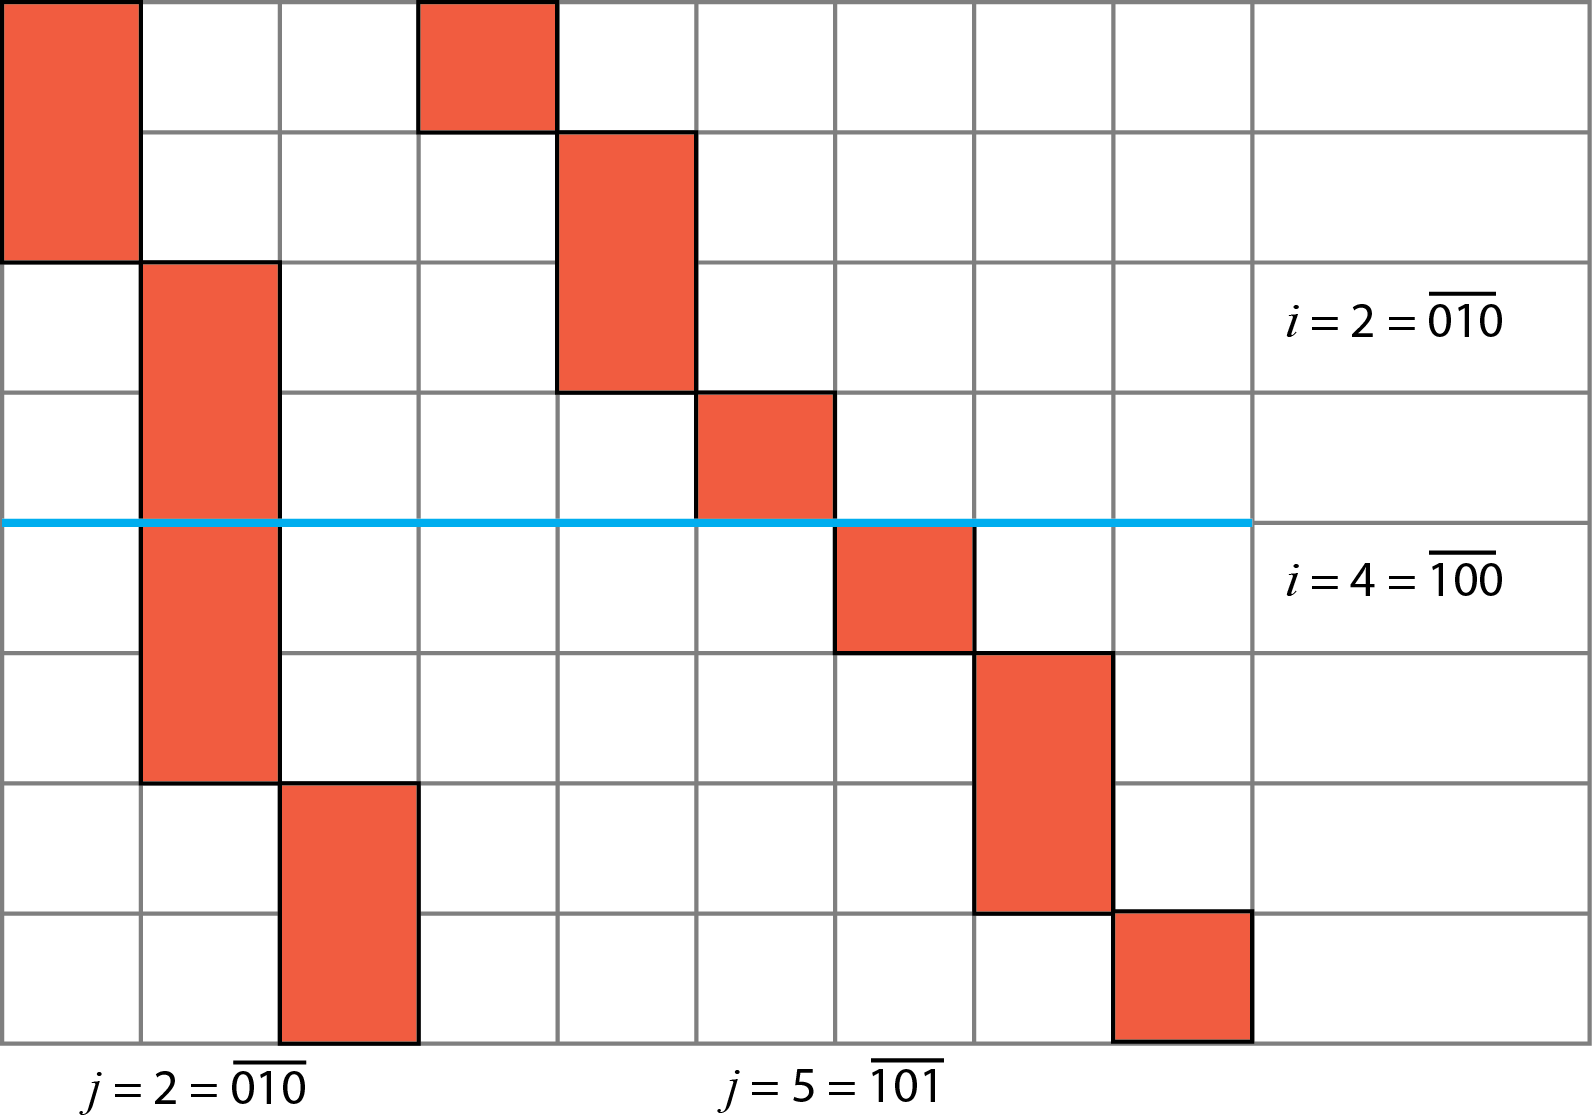
\includegraphics[width=0.7\textwidth]{part1_img/pattern_structure}
  \caption{Хафовские паттерны скоса.}
\label{fig:patterns}

Последняя цифра $j$ отвечает за наличие  дополнительного сдвига половинок на пиксель.
Первая цифра $i$ отвечает за выбор верхней или нижней частей.
\end{figure}

Теперь рассмотрим свойства двоичного представления другого индекса $i = \overline{i_1 i_2 \dots i_n}$, отвечающего номеру строки изображения, которую нужно сдвинуть.
Первая цифра $i_1$ показывает, меньше ли $i$ чем $2^{n-1}$, т. е. находится ли эта строка выше или ниже середины.
Если строка выше середины, то она соответствует верхней половине паттерна $j$, поэтому величина сдвига такая же, как для $\hat{j} = \overline{j_1\dots j_{n-1}}$ и $\tilde{i} = \overline{i_2\dots i_{n}}$.
Иначе величину сдвига нужно увеличить на $pattern_{\hat{j}}[2^{n-1}] + j_n = \hat{j} + j_n$ (см. рис. ~\ref{fig:patterns}):
\begin{equation}\notag
pattern_j[i] = 
\begin{cases}
pattern_{\hat{j}}[\tilde{i}], &\text{если $i_1 = 0$},\\
\hat{j} + j_n + pattern_{\hat{j}}[\tilde{i}], &\text{если $i_1 = 1$}.
\end{cases}
\end{equation}

Итак, можно написать, что:
\begin{equation}
\begin{aligned}\notag
pattern_j[i] = i_1(\hat{j} + j_n)+  pattern_{\hat{j}}[\tilde{i}] = \dots =\sum_{k = 1}^{n-1}{i_k\overline{j_1 j_2 \dots j_{n-k}}}\ +  \sum_{k = 1}^{n}{i_kj_{n-k+1}} =  \\ 
= \sum_{k = 1}^{n-1}{i_k(2^{n-k-1}j_1 + 2^{n-k-2}j_2 + \dots + j_{n-k})}+  \sum_{k = 1}^{n}{i_k j_{n-k+1}} = \\
= \sum_{k = 1}^{n-1}\sum_{m =1}^{n - k}{2^{n-k-m}i_kj_m} +  \sum_{k = 1}^{n}{i_kj_{n-k+1}}.
\end{aligned}
\end{equation}
Второе слагаемое, очевидно, симметрично относительно перестановки $i$ и $j$.
То же можно сказать и о первом слагаемом:
\begin{equation}\notag
\sum_{k = 1}^{n-1}\sum_{m =1}^{n - k}{2^{n-k-m}i_kj_m} = \sum_{\substack{k,m > 0 \\ k + m \leq n}}{2^{n-(k+m)}i_kj_m}.
\end{equation}
Показана истинность утверждения (\ref{statement1}), а значит, и теорема доказана.
\end{proof}

Итак, было показано, что вычислить поправку $\Delta \textbf f$ можно путем двух последовательных применений преобразования Хафа: сначала для вычисления невязки, а потом для вычисления суммы (\ref{eq:sum_res}).
Таким образом, сложность итерации оценивается как $O(n^2 \log n)$, где $n$ --- линейный размер восстанавливаемого изображения.

\section{Исследование поведения алгоритма}
На рис. ~\ref{fig:time_30it} изображена зависимость времени работы 30 итераций алгоритма, аппроксимированная функцией $C n^2 \log n$, при разных размерах изображения исходного фантома.

\begin{figure}[h!]
  \centering
    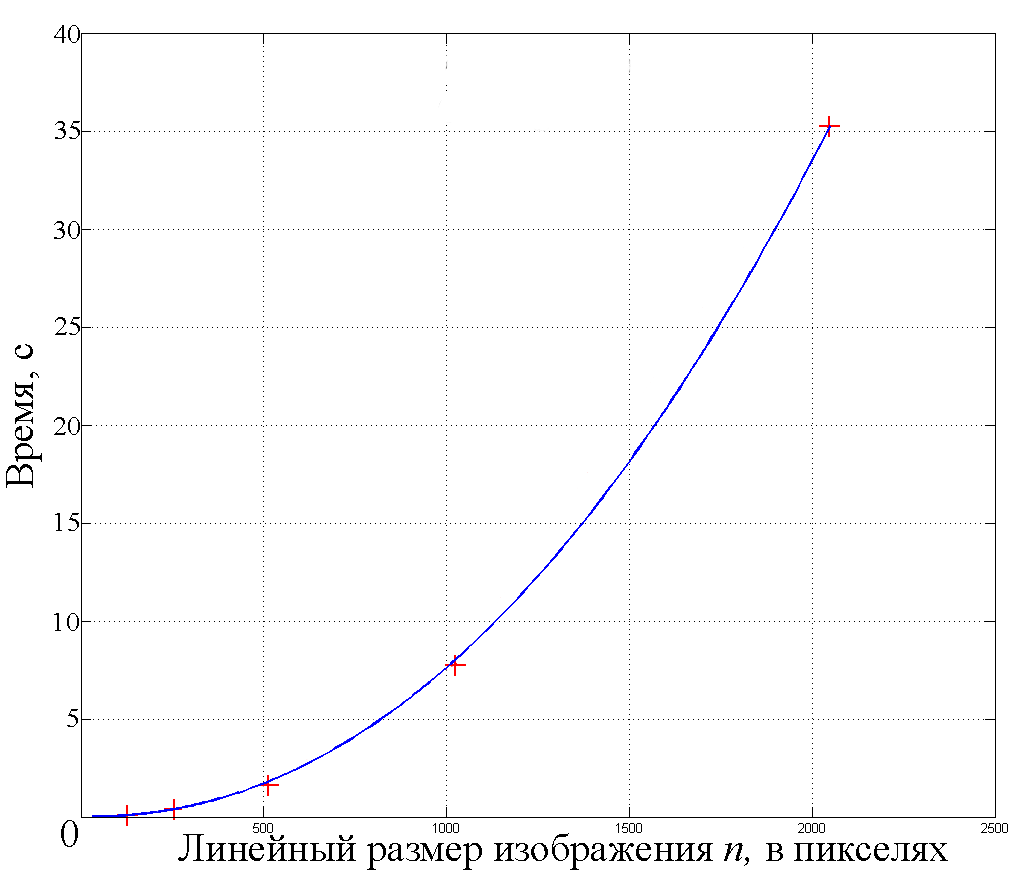
\includegraphics[width=0.7\textwidth]{part1_img/time_30_it}
  \caption{Время работы 30 итераций алгоритма.}
Линией изображена функция $Cn^2\log n$, крестами обозначено измеренное время работы.
\label{fig:time_30it}
\end{figure}

Было исследовано и количество итераций до достижения наперед заданной среднеквадратичной ошибки синограммы в зависимости от размера восстанавливаемого изображения (см. рис. \ref{fig:ris5},a).
Исследуемая величина уменьшается с увеличением размера, так как при большем размере изображения-фантома полное количество углов в БПХ становится больше, т. е. появляется возможность измерить более точную синограмму модели.

\begin{figure}
\begin{subfigure}[h]{0.45\textwidth}
  \centering
    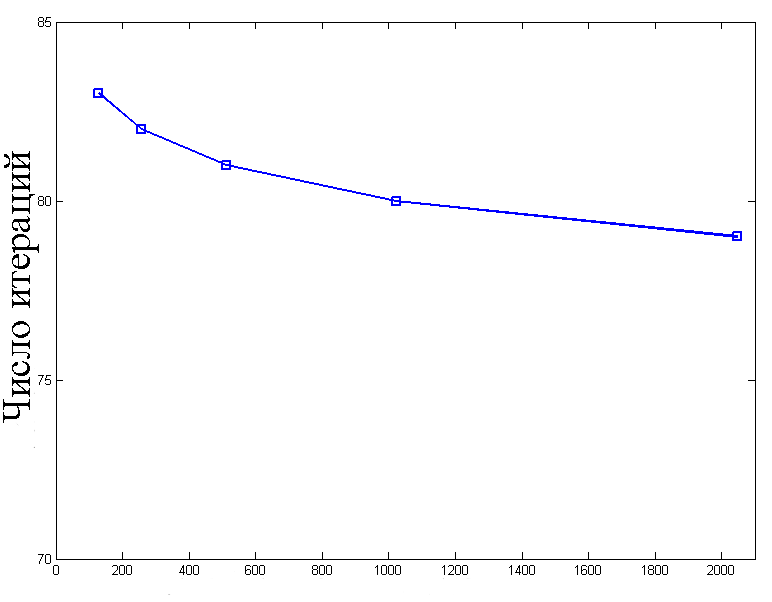
\includegraphics[width=\textwidth]{part1_img/it_till_stop}
    Линейный размер изображения
\label{fig:it_till_stop}
\end{subfigure}

\begin{subfigure}[h]{0.45\textwidth}
  \centering
    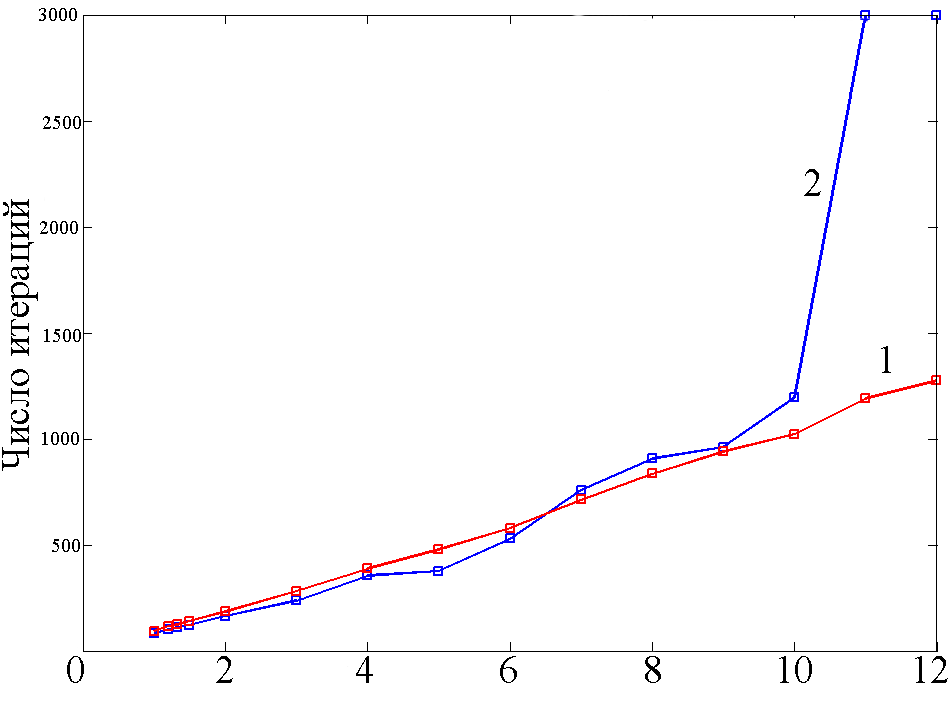
\includegraphics[width=\textwidth]{part1_img/median_correct}
  Степень разрежения
\label{fig:median_reg}
\end{subfigure}
  \caption{Количество итераций до останова.}
\label{fig:ris5}
\end{figure}

Критерием останова в этом и в других экспериментах было достижение некоторой наперед заданной ошибки в преобразовании Хафа по среднеквадратичной метрике:

\begin{equation}\notag
\text{ошибка} = \frac{1}{M}\sum_{i = 1}^{M}{(p_i - \text{Хаф}(\textbf{f})_i)^2}.
\end{equation}

Рассмотренная зависимость была снята при наличии всех $4n-3$ проекций, т. е. полного преобразования Хафа.
В условиях реального эксперимента снять такое количество проекций не представляется возможным.
Действительно, уже для изображения $256\times 256$ пикселей потребовалось бы измерение $4n - 3 = 1021$ разных углов.
Поэтому при работе с реальными данными на входе алгоритма преобразование Хафа будет разреженным.
Время работы при этом останется таким же (в этом смылсе предлагаемый алгоритм проигрывает обычным алгебраическим методам).
Поэтому было исследовано поведение алгоритма при различном разрежении синограммы (см рис. \ref{fig:ris5},б).
На приведённых зависимостях степень разрежения $k$ означает, что для восстановления было использовано в $k$ раз меньше строчек, чем есть в БПХ.

\section{Регуляризация} \label{sect1_2}

При большом разрежении БПХ качество восстановления ухудшается --- недостаточность входных данных порождает шумы на восстановленной картине.
Для корректировки восстанавливаемого изображения применялась регуляризация --- сглаживающий фильтр с сохранением границ после каждой итерации.
Приведённые зависимости были сняты с использованием медианного фильтра размера $3 \times 3$ для изображения размером $256 \times 256$.
На рис. \ref{fig:ris5},б цифрой 1 обозначена зависимость с использованием медианного фильтра, цифрой 2 --- без.

Поведение итерационной процедуры при различном разрежении также отражают рис. \ref{fig:conv_all}.
На них изображено поведение логарифма среднеквадратичной ошибки восстанавливаемого изображения в пределах 5000 итераций.

\begin{equation}\notag
\text{ошибка} = \frac{1}{N}\sum_{j = 1}^{N}{(f^\text{фантом}_j - f_j)^2},
\end{equation}
где через $f^\text{фантом}_j$ обозначен пиксель идеального изображения, а через $f_j$ --- пиксель текущего.

\begin{figure}
\begin{subfigure}[h]{0.45\textwidth}
\centering
  \caption{}
    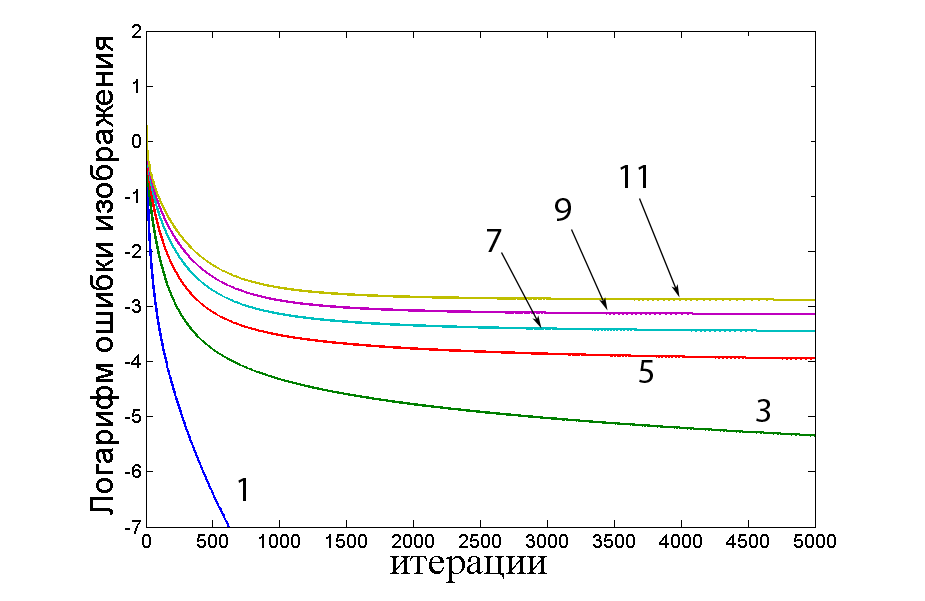
\includegraphics[width=\textwidth]{part1_img/raw}
\label{fig:conv_raw}
\end{subfigure}
~
\begin{subfigure}[h]{0.45\textwidth}
  \centering
  \caption{}
    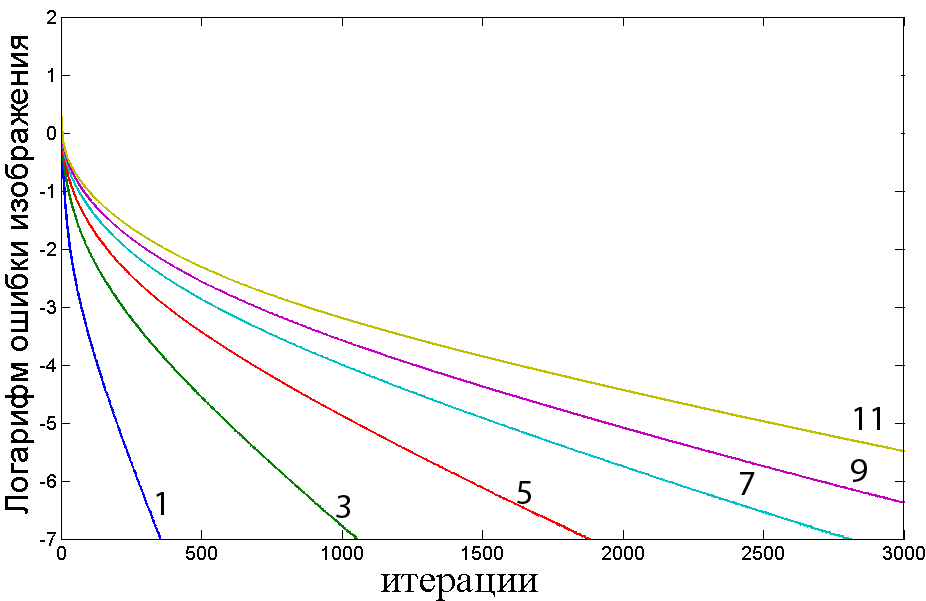
\includegraphics[width= \textwidth]{part1_img/medk}
\label{fig:conv_med}
\end{subfigure}
  \caption{Зависимость среднеквадратичной ошибки изображения от числа итераций.}
%  \centering
Число рядом с кривой соответствует степени разрежения. а --- Без регуляризации, б --- Медианная регуляризация.
\label{fig:conv_all}
\end{figure}

\todo{вставить текст статьи в Кристаллографию-2013}
\todo{вставить текст исследований про регуляризацию по Тихонову}
\todo{..исследовать L1, L0-регуляризаторы..?}

\section{Выводы}
В главе рассмотрена модификация алгебраического метода восстановления компьютерной томографии.
С помощью использования приближения бесконечно тонких рентгеновских лучей для дискретного изображения удается применить быстрое преобразование Хафа (БПХ) в качестве оператора генерации лучевых сумм.
Доказана возможность использовать БПХ не только для подсчета невязки преобразования Хафа, но и для вычисления поправки к изображению в итерационной схеме.
Последнее означает, что асимптотическое время, требуемое для вычисления одной итерации алгебраического метода, можно снизить, применив БПХ, с $O(n^3)$ до $O(n^2 \log n)$ от линейного размера изображения.

Представлены результаты численных экспериментов, описывающие поведение алгоритма в различных условиях.
Для недостаточно полных или зашумленных данных исследована возможность применения регуляризации.
Среди опробованных регуляризаторов на симуляциях сравниваются: медианный и билатеральный фильтры на этапе постобрбаотки и каждой итерации, $L_2$ регуляризация по Тихонову.
Приводятся характер поведения ошибки восстановления на модельных данных от количества итераций и параметров регуляризаторов.
